\documentclass{article}

\usepackage{tikz}
\usetikzlibrary{er, positioning}

\title{Schema ER}
\author{Pietro Jomini}
\date{Maggio 2021}

\begin{document}

\pagenumbering{gobble}
\maketitle
\newpage

\begin{center}
    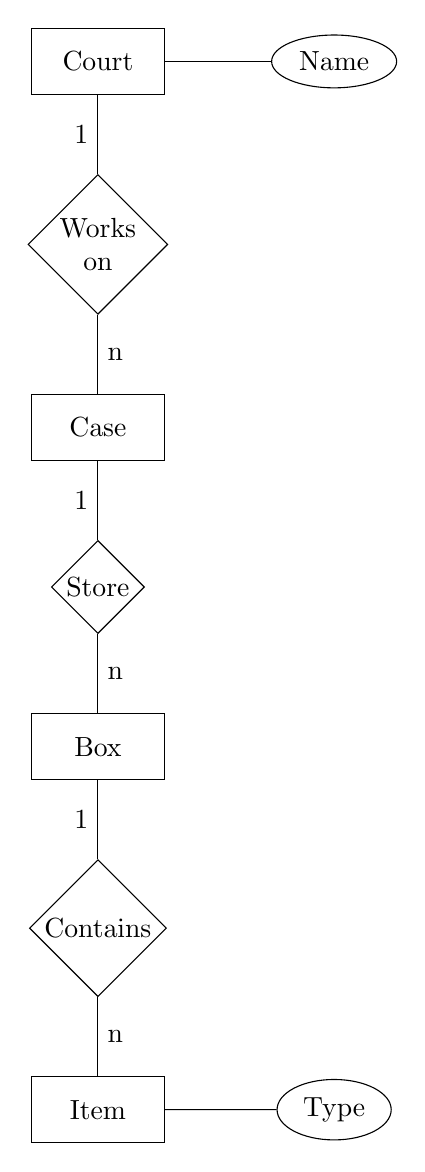
\begin{tikzpicture}[auto, node distance=1cm]

        \node[entity] (court) {Court}
        [grow=right, level distance=3cm]
        child {node[attribute] {Name}};

        \node[relationship] (court_case) [below = of court, align=center] {Works\\on};
        \node[entity] (case) [below = of court_case] {Case};
        \node[relationship] (case_box) [below = of case] {Store};
        \node[entity] (box) [below = of case_box] {Box};
        \node[relationship] (box_item) [below = of box] {Contains};

        \node[entity] (item) [below = of box_item] {Item}
        [grow=right, level distance=3cm]
        child {node[attribute] {Type}};

        \path(court_case) edge node {1} (court) edge node {n} (case);
        \path(case_box) edge node {1} (case) edge node {n} (box);
        \path(box_item) edge node {1} (box) edge node {n} (item);

    \end{tikzpicture}
\end{center}
\end{document}
